\documentclass[12pt,a4paper]{report}

\usepackage[utf8]{inputenc}
\usepackage[T1]{fontenc}
\usepackage[italian]{babel}
\usepackage{lmodern}
\usepackage{microtype}
\usepackage{titlesec}
\usepackage{graphicx}
\usepackage{float}
\usepackage{xcolor}
\usepackage{caption}
\usepackage{enumitem}
\usepackage{xurl}
\usepackage[htt]{hyphenat}
\usepackage{parskip}
\usepackage{tabularx}
\usepackage{array}
\usepackage{lineno} % Pacchetto per la numerazione automatica delle righe fisiche
\usepackage{framed}

% 1. MARGINI RIDOTTI (sfrutta più spazio nella pagina)
\usepackage[
  top=2.2cm,
  bottom=2.2cm,
  left=2.5cm,
  right=2.5cm
]{geometry}

\definecolor{captiongray}{RGB}{70, 70, 70}
\captionsetup[figure]{
    font=small,
    labelfont={color=captiongray},
    textfont={color=captiongray},
    justification=centering
}

% 2. TITOLO CAPITOLO (Grande "\huge" e senza punto dopo il numero)
\titleformat{\chapter}[hang]
    {\normalfont\huge\bfseries}
    {\thechapter}
    {0.75em}
    {}

% 3. POSIZIONAMENTO IN ALTO (Rimuove lo spazio vuoto enorme sopra il capitolo)
\titlespacing*{\chapter}{0pt}{-15pt}{15pt}
\titlespacing*{\section}{0pt}{12pt}{6pt}

\usepackage[hidelinks]{hyperref}
\hypersetup{
    linktoc=all,
    pdftitle={HearthCode},
    pdfauthor={Simone Marsili, Francesco Dama}
}

\begin{document}

\pagenumbering{gobble}
\begin{titlepage}
    \centering
    {\Large Relazione per Basi di Dati\par}

    \vspace{1cm}

    {\Huge\bfseries Dalla Ricetta Al Carrello - Sistema di gestione ricette, acquisti e promozioni\par}

    \vfill

    \begin{flushright}
        Simone Marsili\\
        Francesco Dama
    \end{flushright}
\end{titlepage}

\clearpage
\pagenumbering{Roman}
\tableofcontents

\clearpage
\pagenumbering{arabic}
\chapter{Analisi}

\section{Analisi dei requisiti}

Si vuole realizzare un database a supporto della gestione di un ricettario online, il quale mette a disposizione la possibilità di acquisto. 
La base di dati dovrà quindi immagazzinare informazioni relative agli utenti, alle ricette da loro pubblicate, nonché agli ordini effettuati 
sul sito. Gli amministratori potranno dunque consultare tutte le ricette inserite, aggiungere nuovi ingredienti disponibili e lanciare nuove 
promozioni.


\textbf{\\Intervista}


Si vuole tenere traccia degli utenti registrati al sito memorizzandone nome, cognome, codice fiscale, email, password e opzionalmente un indirizzo di spedizione.
In seguito alla registrazione l’utente può visualizzare e/o creare delle ricette.
\\Chi crea una ricetta vi deve associare un nome, una descrizione della preparazione, un tempo stimato di preparazione e i necessari ingredienti con le relative quantità (espresse in grammi).
\\Gli ingredienti disponibili al momento della creazione della ricetta sono quelli presenti sul sito, ognuno associato ad un codice identificativo, un nome e un relativo prezzo al chilo.
\\Inoltre nel creare la ricetta, l’utente deve associarla a una o più categorie, anche queste visualizzabili nel sito: ogni categoria è costituita da un codice univoco, una descrizione e un nome (vegano, vegetariano, italiano, asiatico, ...).
\\Gli utenti possono per di più lasciare delle recensioni alle ricette sul sito, indicando un voto in una scala da 1 a 10 e un eventuale consiglio di modifica (un utente può scrivere un solo giudizio per una determinata ricetta).
\\In aggiunta, il sistema mette a disposizione la possibilità di acquisto: un utente che visualizza una ricetta può acquistare tutto il necessario per prepararla a casa (eventualmente un utente può acquistare più di una ricetta nello stesso ordine).
\\Il costo di una ricetta è calcolato quindi come somma dei costi degli ingredienti valutandone il peso.
Per semplicità non viene gestita la disponibilità degli ingredienti in magazzino.
\\Infine il sito può lanciare delle promozioni periodiche che offrono degli sconti: in particolare la percentuale di sconto riferita ad una specifica promo dipende dalla categoria di ricetta.
Nel caso una ricetta preveda più sconti al momento dell’acquisto (più categorie scontate), verrà applicato quello maggiore.


\textbf{\\Revisione}

A seguito dell’analisi dell’intervista e del confronto del dominio con applicazioni e siti web realmente esistenti, si è deciso di apportare alcuni cambiamenti nella modellazione e gestione degli sconti, in modo tale da renderle più complesse e realistiche. 
\\\\Una prima modifica proibisce all’utente di pubblicare due ricette con lo stesso nome, in modo tale da prevenire duplicazioni di ricette sul sito.
\\\\Una seconda modifica è riassunta dalla seguente descrizione: “la percentuale di sconto riferita ad una specifica promo dipende dalla categoria di ricetta e dal numero di ingredienti di quest’ultima”.
Nello specifico, uno sconto si riferisce ad un certo intervallo di numero di ingredienti, e una ricetta per essere scontata deve avere un numero di ingredienti appartenente a questo range, oltre che appartenere alla specifica categoria interessata.
\\\\Infine il dominio impone il seguente vincolo: i range di ingredienti di eventuali sconti riferiti ad una stessa categoria e stessa promozione non devono essere sovrapposti.

A seguito delle revisioni si riformula l’intervista nella seguente:

\begin{table}[H]
\centering
\setlength{\extrarowheight}{2pt}
\begin{tabularx}{\textwidth}{|c|X|}
\hline
\multicolumn{2}{|c|}{\textit{\textbf{Definizione delle specifiche in linguaggio naturale}}} \\
\hline
1 & Si vuole tenere traccia degli utenti registrati al sito memorizzando nome, cognome,\\
2 & codice fiscale, email, password e opzionalmente un indirizzo di spedizione. \\
3 & In seguito alla registrazione l'utente può visualizzare e/o creare delle ricette. \\
4 & Chi crea una ricetta vi deve associare un nome, una descrizione della preparazione, \\
5 & un tempo stimato di preparazione e i necessari ingredienti con le relative quantità \\
6 & (espresse in grammi). \\
7 & Gli ingredienti disponibili al momento della creazione della ricetta sono quelli \\
8 & presenti sul sito, ognuno associato ad un codice identificativo, un nome e un relativo \\
9 & prezzo al chilo. \\
10 & Inoltre nel creare la ricetta, l'utente deve associarla a una o più categorie, anche \\
11 & queste visualizzabili nel sito: ogni categoria è costituita da un codice univoco, una \\
12 & descrizione e un nome (vegano, vegetariano, italiano, asiatico, ...). \\
13 & Il sistema proibisce all'utente di pubblicare più ricette con lo stesso nome. \\
14 & Gli utenti possono per di più lasciare delle recensioni alle ricette sul sito, indicando \\
15 & un voto in una scala da 1 a 10 e un eventuale consiglio di modifica (un utente può \\
16 & scrivere un solo giudizio per una determinata ricetta). \\
17 & In aggiunta, il sistema mette a disposizione la possibilità di acquisto: un utente \\
18 & che visualizza una ricetta può acquistare tutto il necessario per prepararla a casa \\
19 & (eventualmente un utente può acquistare più di una ricetta nello stesso ordine). \\
20 & Il costo di una ricetta è calcolato quindi come somma dei costi degli ingredienti \\
21 & valutandone il peso. \\
22 & Per semplicità non viene gestita la disponibilità degli ingredienti in magazzino. \\
23 & Infine il sito può lanciare delle promozioni periodiche che offrono degli sconti: \\
24 & in particolare la percentuale di sconto riferita ad una specifica promo dipende \\
25 & dalla categoria di ricetta e dal numero di ingredienti di quest'ultima: un singolo \\
26 & sconto copre un certo range di numero di ingredienti, e i range di ingredienti di \\
27 & eventuali sconti riferiti ad una stessa categoria e stessa promozione non devono \\
28 & essere sovrapposti. \\
29 & Nel caso una ricetta preveda più sconti al momento dell'acquisto (più categorie \\
30 & scontate e/o più sconti per una singola categoria), verrà applicato quello maggiore. \\
\hline
\end{tabularx}
\caption*{\textbf{Tabella 1.1.1} - \textit{Specifiche di progetto in linguaggio naturale.}}
\end{table}

Si procede con l'individuare i termini principali che riassumono al meglio i concetti del dominio.

\begin{table}[H]
\centering
\renewcommand{\arraystretch}{1.3} % Mantiene un po' di respiro tra le righe
\setlength{\tabcolsep}{8pt}

\begin{tabularx}{\textwidth}{|l|X|}
\hline
\textbf{Termine} & \textbf{Breve descrizione} \\
\hline
Utente & Colui che naviga sul sito e che può visualizzare, pubblicare, recensire e acquistare ricette. \\
Ricetta & Elemento acquistabile che rappresenta un piatto, pensato per essere preparato e consumato. \\
Ingrediente & Oggetto necessario per la preparazione di una ricetta. \\
Categoria & Gruppo di appartenenza di una ricetta secondo un determinato criterio. \\
Recensione & Feedback virtuale riguardante una ricetta e pubblicato da un utente. \\
Ordine & Richiesta d’acquisto che raggruppa una o più ricette selezionate. \\
Promozione & Evento commerciale periodico vantaggioso per gli utenti che desiderano acquistare ricette. \\
Sconto & Ribasso del prezzo di una ricetta secondo certi requisiti. \\
\hline
\end{tabularx}
\caption*{\textbf{Tabella 1.1.2} - \textit{Glossario dei termini.}}
\end{table}


Si tiene conto delle seguenti correzioni di ambiguità:

\begin{table}[H]
\centering
\renewcommand{\arraystretch}{1.3} % Mantiene lo spazio verticale comodo per il testo
\setlength{\tabcolsep}{8pt}      % Distanzia il testo dai bordi laterali

\begin{tabularx}{\textwidth}{|c|l|X|}
\hline
\textbf{Riga} & \textbf{Termine} & \textbf{Nuovo termine} \\
\hline
16 & Giudizio & Recensione \\
18 & …tutto il necessario… & Ingredienti \\
24 & Promo & Promozione \\
\hline
\end{tabularx}
\caption*{\textbf{Tabella 1.1.3} - \textit{Rilevamento delle ambiguità e correzioni proposte.}}
\end{table}


\begin{table}[H]
\centering
\setlength{\extrarowheight}{2pt}
\begin{tabularx}{\textwidth}{|c|X|}
\hline
\multicolumn{2}{|c|}{\textit{\textbf{Secifiche ristrutturate}}} \\
\hline
1 & Degli \textbf{utenti} registrati al sito si memorizzano nome, cognome, codice fiscale, email, \\
2 & password e opzionalmente un indirizzo di spedizione. \\
3 & L’utente può visualizzare e/o creare delle ricette. \\
4 & Chi crea una \textbf{ricetta} vi deve associare un nome, una descrizione della preparazione, \\
5 & un tempo stimato di preparazione e ogni \textbf{ingrediente} necessario con le relative \\
6 & quantità (espresse in grammi). \\
7 & Gli ingredienti disponibili al momento della creazione della ricetta sono quelli \\
8 & presenti sul sito, ognuno associato ad un codice identificativo, un nome e un relativo \\
9 & prezzo al chilo. \\
10 & Inoltre nel creare la ricetta, l’utente deve associarla a una o più categorie, anche \\
11 & queste visualizzabili nel sito: ogni \textbf{categoria} è costituita da un codice univoco, \\
12 & una descrizione e un nome (vegano, vegetariano, italiano, asiatico, ...). \\
13 & Il sistema proibisce all’utente di pubblicare più ricette con lo stesso nome. \\
14 & Per una determinata ricetta presente sul sito, un utente può pubblicare al massimo \\
15 & una recensione, indicando un voto in una scala da 1 a 10 e un eventuale consiglio \\
16 & di modifica. \\
17 & Un utente che visualizza una ricetta può inoltre acquistare l’insieme di tutti gli \\
18 & ingredienti per prepararla a casa (eventualmente un utente può acquistare gli \\
19 & ingredienti di più ricette nello stesso ordine). \\
20 & Il costo di una ricetta è calcolato quindi come somma dei costi degli ingredienti \\
21 & valutandone il peso. \\
22 & Per semplicità non viene gestita la disponibilità degli ingredienti in magazzino. \\
23 & Infine il sito può lanciare delle \textbf{promozioni} periodiche che offrono degli \textbf{sconti}:\\
24 & in particolare la percentuale di sconto riferita ad una specifica promo dipende \\
25 & dalla categoria di ricetta e dal numero di ingredienti di quest’ultima: un singolo \\
26 & sconto copre un certo range di numero di ingredienti, e i range di ingredienti di \\
27 & eventuali sconti riferiti ad una stessa categoria e stessa promozione non devono \\
28 & essere sovrapposti. \\
29 & Nel caso una ricetta preveda più sconti al momento dell’acquisto (più categorie \\
30 & scontate e/o più sconti per una singola categoria), verrà applicato quello maggiore. \\
\hline
\end{tabularx}
\caption*{\textbf{Tabella 1.1.4} - \textit{Specifiche di progetto ristrutturate ed estrazione dei concetti principali.}}
\end{table}


\section{Analisi delle viste}

A seguito delle specifiche ristrutturate, si divide il DataBase in due tipologie di utenti diverse:

\begin{itemize}
    \item \textbf{Utente standard}
    \item \textbf{Amministratore}
\end{itemize}

\subsection{Utenti standard}

I requisiti relativi agli utenti standard sono stati già descritti nel paragrafo precedente e non necessitano di alcuna aggiunta.

\textbf{Elenco delle principali azioni per gli utenti standard:}\\

\begin{enumerate}[label=\textbf{U\arabic* - }, leftmargin=1.2cm, itemsep=0.8em]

    \item REGISTRAZIONE UTENTE\\
    L’utente deve essere in grado di registrarsi correttamente al sito.

    \item VISUALIZZAZIONE DELLE RICETTE\\
    L’utente deve poter essere in grado di visualizzare l’elenco di tutte le ricette pubblicate sul sito.

    \item VISUALIZZAZIONE DI RICETTE PER FILTRO\\
    L’utente deve poter visualizzare delle ricette secondo dei filtri di ricerca adeguati:
    \begin{enumerate}[label=\textbf{U3.\arabic* - }, leftmargin=1.2cm, itemsep=0.2em, topsep=0.3em]
        \item Filtro per nome della ricetta
        \item Filtro per ingrediente
        \item Filtro per tempi di preparazione inferiori a un dato limite
        \item Filtro per prezzo
        \item Filtro per utente
        \item Filtro per categoria/e
    \end{enumerate}

    \item VISUALIZZAZIONE INGREDIENTI\\
    L’utente può visualizzare gli ingredienti disponibili sul sito che possono essere usati per comporre le ricette.

    \item PUBBLICAZIONE DI UNA RECENSIONE\\
    L’utente può valutare una data ricetta pubblicando una recensione contenente voto da 1 a 10 e opzionalmente un commento/suggerimento di modifica.

    \item PUBBLICAZIONE DI UNA RICETTA\\
    L’utente deve poter essere in grado di pubblicare una ricetta sul sito, selezionando gli ingredienti necessari per realizzarla, la/le categoria/e a cui appartiene e i vari attributi.

    \item VISUALIZZAZIONE VANTAGGI\\
    L’utente può visualizzare le categorie di ricette per cui ci sono sconti attivi.

    \item VISUALIZZAZIONE ECCELLENZE\\
    L’utente può visualizzare:
    \begin{enumerate}[label=\textbf{U8.\arabic* - }, leftmargin=1.2cm, itemsep=0.2em, topsep=0.3em]
        \item Le migliori ricette in base alle recensioni
        \item I migliori utenti in base alla media delle recensioni delle ricette da loro pubblicate
        \item Le ricette maggiormente ordinate
        \item Le categorie di ricette maggiormente ordinate
    \end{enumerate}

    \item EFFETTUAZIONE DI UN ORDINE\\
    L’utente può richiedere un ordine, il quale contiene il set di ingredienti di una o più ricette. All’ordine vengono applicati eventuali sconti (ad una ricetta che ha più sconti possibili verrà applicato quello massimo).

    \item VISUALIZZAZIONE STORICO ORDINI\\
    L’utente può visualizzare tutti i suoi ordini effettuati in passato negli ultimi $n$ mesi, in base alle sue preferenze.

    \item VISUALIZZAZIONE SPECIFICA RICETTA\\
    L’utente può visualizzare tutti i dettagli di una specifica ricetta, come il prezzo, l’utente che l’ha pubblicata, la media delle recensioni, l’elenco degli ingredienti e le categorie di appartenenza.

\end{enumerate}

\subsection{Amministratore}

L’amministratore è colui che si occupa di gestire il sito e i relativi dati, preoccupandosi di registrare i nuovi utenti con le relative informazioni.\\
E’ responsabile della gestione del catalogo di ingredienti disponibili, deve quindi poter inserire nuovi ingredienti determinandone il prezzo al chilo.\\
L’amministratore deve inoltre poter inserire nuove categorie di ricetta in base allo sviluppo culinario nel mondo.\\
Deve inoltre tenere sotto controllo l’equilibrio economico del sito, aggiungendo opportunamente nuove promozioni e sconti associati.\\
Infine l’amministratore deve mantenere il sito pulito e coerente: egli ha infatti il potere di rimuovere utenti che hanno pubblicato ricette con dati inadeguati.

\textbf{Elenco delle principali azioni per l'amministratore:}\\

\begin{enumerate}[label=\textbf{A\arabic* - }, leftmargin=1.2cm, itemsep=0.8em]

    \item INSERIMENTO INGREDIENTE\\
    L’amministratore deve poter aggiungere un ingrediente alla lista disponibile, specificando il prezzo al chilo.

    \item AGGIORNAMENTO INGREDIENTE\\
    L’amministratore può modificare il prezzo (al chilo) per un ingrediente disponibile sul sito.

    \item INSERIMENTO CATEGORIA\\
    L’amministratore può aggiungere nuove categorie di ricette disponibili sul sito.

    \item LANCIO DI UNA PROMOZIONE\\
    L’amministratore può inserire nuove promozioni periodiche che annunciano l’inizio di un periodo vantaggioso.

    \item PUBBLICAZIONE SCONTI\\
    L’amministratore può inserire nuovi sconti in base alla promozione di riferimento e alla categoria di ricetta.

    \item RIMOZIONE UTENTI\\
    L’amministratore può rimuovere manualmente utenti che hanno pubblicato diverse ricette con categorie inadeguate. \\
    Il sistema pone particolare attenzione alle ricette vegane e l’amministratore è in grado di individuare in modo automatico ricette classificate come tali ma che non lo sono (ad esempio una ricetta classificata come vegana ma che contiene carne o pesce). In questo particolare caso delle ricette vegane, l’utente verrà rimosso dal sistema alla pubblicazione di almeno 3 ricette inadeguate (e tutte le sue ricette con lui).

\end{enumerate}
\chapter{Progettazione concettuale}

\section{Utenti standard}

\subsection{Gestione pubblicazione ricette}

\begin{figure}[H]
    \centering
    % Regola la larghezza. 0.8\textwidth significa "80% della larghezza del testo".
    % Puoi usare anche cm, es: width=10cm
    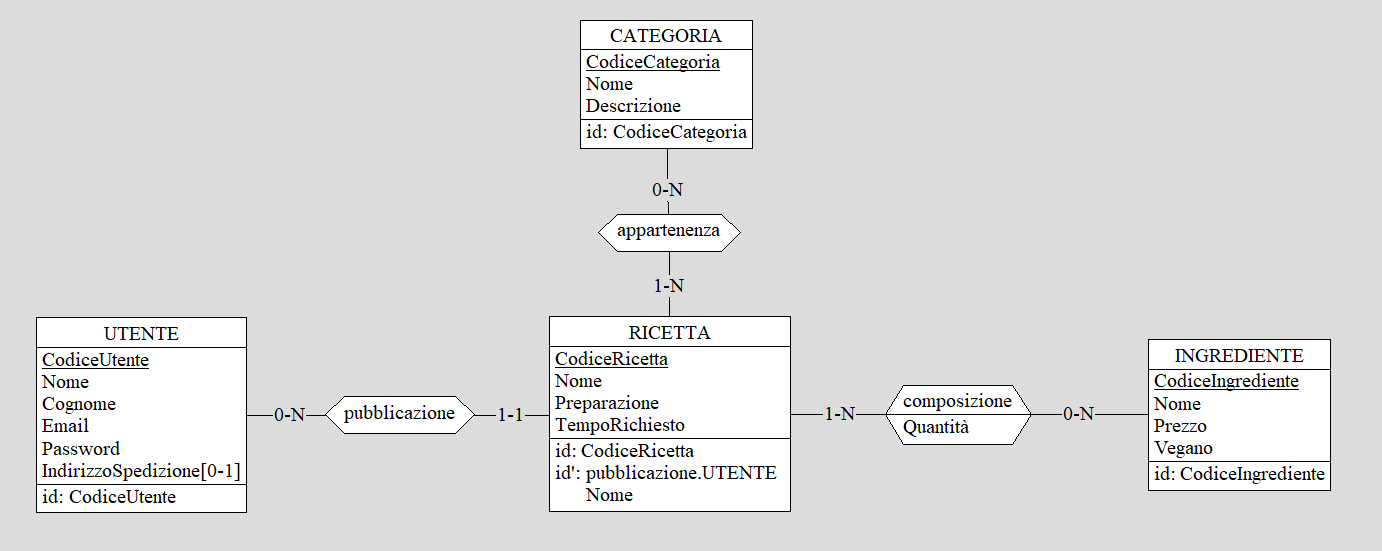
\includegraphics[width=1\textwidth]{images/conc_pubblicazione.png}
    \caption{Schema scheletro per la pubblicazione ricette}
    \label{fig:pubbl} % Etichetta per fare riferimento: vedi Figura \ref{fig:mia_immagine}
\end{figure}


Secondo il nostro dominio, un \textbf{utente} al momento della registrazione deve inserire obbligatoriamente le sue generalità e opzionalmente un indirizzo di spedizione. L’\textbf{utente} quindi rappresenta un’entità fondamentale nel nostro schema concettuale, ed è identificato da un codice univoco (CodiceUtente) assegnato dal sistema in maniera progressiva e automatica al momento della registrazione. Si è deciso di non usare il codice fiscale come identificatore per due motivi principali: 
\begin{itemize}
    \item La maggior parte dei ricettari online non richiede il codice fiscale dell'utente.
    \item Evitare casi estremi di coincidenza di codici fiscali.
\end{itemize}

Un \textbf{utente}, una volta registrato al sito, può pubblicare delle \textbf{ricette},  le quali posseggono un codice univoco progressivo (CodiceRicetta) e un identificatore alternativo (Utente, nomeRicetta) e sono associate a un solo \textbf{utente}, ovvero colui che la pubblica.

Si è deciso in fase di progettazione concettuale di tenere valida la chiave primaria CodiceRicetta, in quanto la chiave alternativa composta (Utente, NomeRicetta) avrebbe portato al pericolo di ridondanze e complicazioni per quanto riguarda un futuro aggiornamento del Database e la sua effettiva propagazione. 
\\L’identificatore alternativo (Utente, nomeRicetta) verrà successivamente espresso come vincolo UNIQUE in fase di progettazione logica, in modo tale da modellare correttamente il vincolo di dominio secondo il quale un \textbf{utente} non può pubblicare ricette omonime.

Al momento della pubblicazione della \textbf{ricetta}, oltre agli attributi generali bisogna associarvi obbligatoriamente almeno un \textbf{ingrediente}, indicando anche la sua relativa quantità, la quale viene salvata nell’associazione \textbf{composizione} come attributo. \\
Dopo aver aggiunto almeno un \textbf{ingrediente} va aggiunta obbligatoriamente almeno una \textbf{categoria} di appartenenza per la \textbf{ricetta}, la quale è identificata da un codice univoco (CodiceCategoria). \\
Gli ingredienti sono identificati da un codice univoco (CodiceIngrediente), in più dispongono di un nome, un prezzo €/Kg e un attributo booleano (Vegano) che chiarisce se un determinato \textbf{ingrediente} sia derivato da animali o meno.

\subsection{Gestione recensioni}

\begin{figure}[H]
    \centering
    % Regola la larghezza. 0.8\textwidth significa "80% della larghezza del testo".
    % Puoi usare anche cm, es: width=10cm
    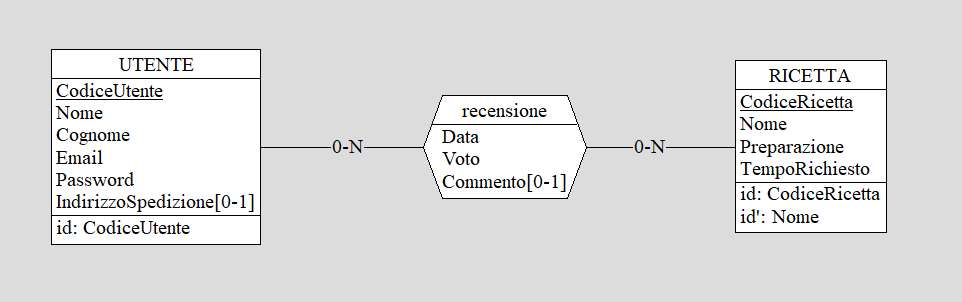
\includegraphics[width=1\textwidth]{images/conc_recensione.png}
    \caption{Schema scheletro per la recensione di ricette}
    \label{fig:recens} % Etichetta per fare riferimento: vedi Figura \ref{fig:mia_immagine}
\end{figure}


Secondo le regole di dominio, un \textbf{utente} può lasciare più recensioni a \textbf{ricette} diverse (non più di una recensione per una stessa ricetta) e una \textbf{ricetta} può avere più \textbf{recensioni} da parte di più \textbf{utenti}.


Inizialmente si era pensato di reificare l’associazione \textbf{recensione} in una entità, ma progredendo nello sviluppo ci si è resi conto che questa entità era composta esclusivamente da identificatori esterni (una recensione poteva essere identificata solamente tramite utente e ricetta a cui era associata), quindi si è optato per renderla un’associazione, in quanto non possono esistere due tuple che abbiano stessi \textbf{utente} e \textbf{ricetta}.

 
L’associazione \textbf{recensione} prevede alcuni attributi obbligatori, come Data e Voto, e un attributo opzionale, ovvero il commento.
Tutto ciò rappresenta come funziona al giorno d’oggi il sistema delle recensioni in approssimativamente tutti i casi.

\subsection{Gestione ordini}

\begin{figure}[H]
    \centering
    % Regola la larghezza. 0.8\textwidth significa "80% della larghezza del testo".
    % Puoi usare anche cm, es: width=10cm
    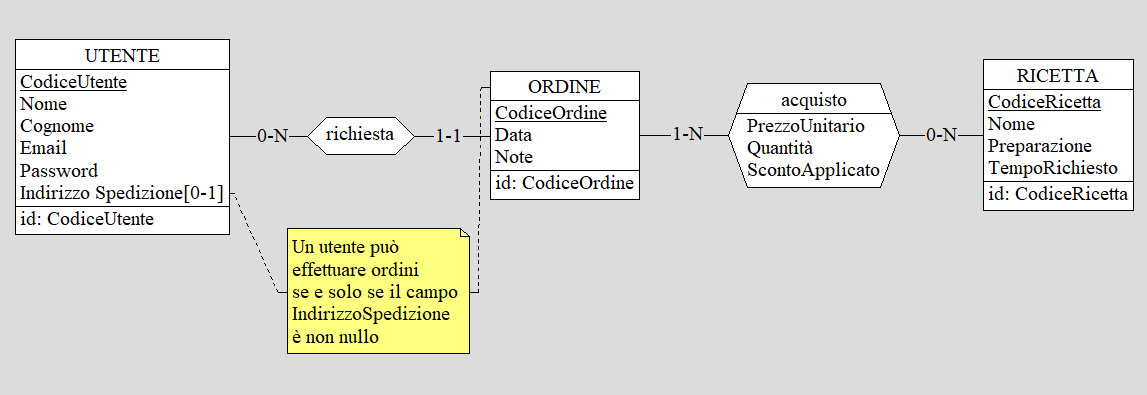
\includegraphics[width=1\textwidth]{images/conc_ordine.png}
    \caption{Schema scheletro per l'ordine di ricette.}
    \label{fig:ord} % Etichetta per fare riferimento: vedi Figura \ref{fig:mia_immagine}
\end{figure}

Per modellare nel modo più corretto il concetto di \textbf{ordine}, si è deciso di reificarlo in un'apposita entità \textbf{ordine}, identificata da un codice progressivo (CodiceOrdine).\\
In questo modo si è potuto storicizzare gli ordini nel sito, i quali vengono così correttamente memorizzati e sono disponibili per apposite interrogazioni che riguardano la storia passata delle \textbf{ricette}.\\
Se si fosse utilizzata una semplice associazione con attributi, non si sarebbe riusciti a modellare questo aspetto e il concetto di \textbf{ordine} come entità viva all’interno del sistema.

Secondo il dominio, l’\textbf{utente} può acquistare il set di tutti gli ingredienti necessari alla ricetta; tuttavia è risultato più efficiente collegare l’ordine direttamente alla \textbf{ricetta}, in modo tale da avere un riferimento diretto a tutti gli ingredienti di cui essa si compone.\\
Non sarebbe stato ugualmente corretto collegare l’\textbf{ordine} all’entità ingrediente in quanto un utente non può scegliere quali ingredienti di una \textbf{ricetta} acquistare e quali no: può decidere solo di ordinare direttamente tutti gli ingredienti necessari (ad esempio come succede sul noto sito web HelloFresh).

L’associazione \textbf{acquisto} è di tipo N a N, in quanto come da dominio, un’\textbf{ordine} può essere effettuato su più ricette e una stessa \textbf{ricetta} può essere ordinata naturalmente in più \textbf{ordini} e da più \textbf{utenti}.\\
L’associazione presenta inoltre l’attributo Quantità per rendere possibile acquistare la stessa \textbf{ricetta} più volte nello stesso ordine; infine gli attributi PrezzoUnitario e ScontoApplicato permettono di congelare al momento dell’\textbf{ordine} il prezzo della singola ricetta e lo sconto per quest'ultima, in quanto dinamici all’interno del sito.

\subsection{Gestione sconti e promozioni}

\begin{figure}[H]
    \centering
    % Regola la larghezza. 0.8\textwidth significa "80% della larghezza del testo".
    % Puoi usare anche cm, es: width=10cm
    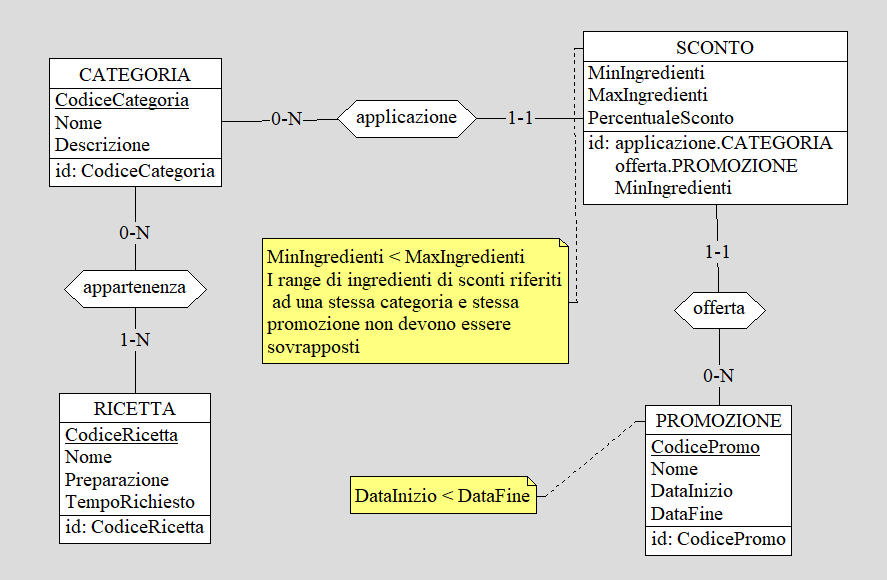
\includegraphics[width=1\textwidth]{images/conc_sconto.png}
    \caption{Schema scheletro per sconti e promozioni.}
    \label{fig:sconto} % Etichetta per fare riferimento: vedi Figura \ref{fig:mia_immagine}
\end{figure}

La \textbf{promozione} è stata modellata come semplice entità, con codice promozionale e range di date per rendere la promo periodica.
Osservando il dominio si è individuata la dipendenza

\textbf{Promozione, Categoria, Range Ingredienti -> Sconto}

E' stato quindi necessario reificare lo \textbf{sconto} in un’entità apposita, identificata dagli attributi/entità da cui essa dipende.\\
Per quanto riguarda il range del numero di ingredienti si è deciso di considerare solo “MinIngredienti” come identificatore, evidenziando i vincoli inespressi come si può notare in figura.

L’associazione \textbf{applicazione} è del tipo 1 a N in quanto uno \textbf{sconto} si riferisce ad una specifica \textbf{categoria}, mentre una \textbf{categoria} può avere più possibili \textbf{sconti} (ad esempio per promozioni e/o range di ingredienti diversi).\\
Infine l’associazione \textbf{offerta} è anch’essa di tipo 1 a N, per ragionamento analogo.


\section{Amministratore}

Nel panorama analizzato si suppone che l’amministratore sia uno solo e che egli sia solamente responsabile di popolare parte del database ed eventualmente di aggiornare i suoi dettagli; per fare ciò non è necessario memorizzare alcun suo dato.
Di conseguenza si è deciso di non tenerne conto nello schema E/R completo.

Si noti che nello schema concettuale finale viene aggiunto un ulteriore attributo “Ruolo” in UTENTE, al solo fine di distinguere gli utenti standard dagli amministratori al momento del login al sito.


\section{Schema concettuale finale}

Per la produzione dello schema concettuale finale si sono utilizzati e uniti gli schemi E/R relativi ai sottoproblemi precedentemente illustrati.

Come ultima modifica allo schema finale si è deciso di inserire due ulteriori attributi booleani:
\begin{itemize}
    \item “Attivo” in UTENTE
    \item “Rimossa” in RICETTA
\end{itemize}
Questi attributi sono stati aggiunti al fine di poter implementare facilmente l’operazione A6 di rimozione utenti.

La scelta di utilizzare una cancellazione logica (tramite attributo booleano) anziché una cancellazione fisica del record è motivata dal fatto che sia UTENTE che RICETTA sono coinvolti in numerose relazioni con altre entità (ORDINE, acquisto, recensione, composizione, ecc.), che nel tempo accumulano un volume rilevante di istanze storiche. \\
Una cancellazione fisica dell'utente o della ricetta comporterebbe la perdita — o la necessità di cancellazione a cascata — di tutti i dati storici ad essi collegati (ordini effettuati, recensioni scritte, ricette pubblicate), compromettendo l'integrità referenziale e la consultabilità dello storico anche da parte di altri utenti non coinvolti nella rimozione.

L'introduzione degli attributi "Attivo" e "Rimossa" consente quindi di:
\begin{itemize}
    \item mantenere l'integrità e la coerenza dei dati storici legati a ordini e recensioni già effettuati;
    \item impedire che un utente rimosso possa autenticarsi o effettuare nuove operazioni (pubblicare ricette, effettuare ordini, scrivere recensioni);
    \item impedire che una ricetta "rimossa" venga mostrata o resa acquistabile ai fini di nuove operazioni, pur restando visibile negli storici già esistenti;
    \item semplificare l'operazione A6, che si riduce a un semplice aggiornamento del valore dell'attributo, evitando la gestione più complessa di eliminazioni a cascata sulle relazioni coinvolte.
\end{itemize}

\begin{figure}[H]
    \centering
    % Regola la larghezza. 0.8\textwidth significa "80% della larghezza del testo".
    % Puoi usare anche cm, es: width=10cm
    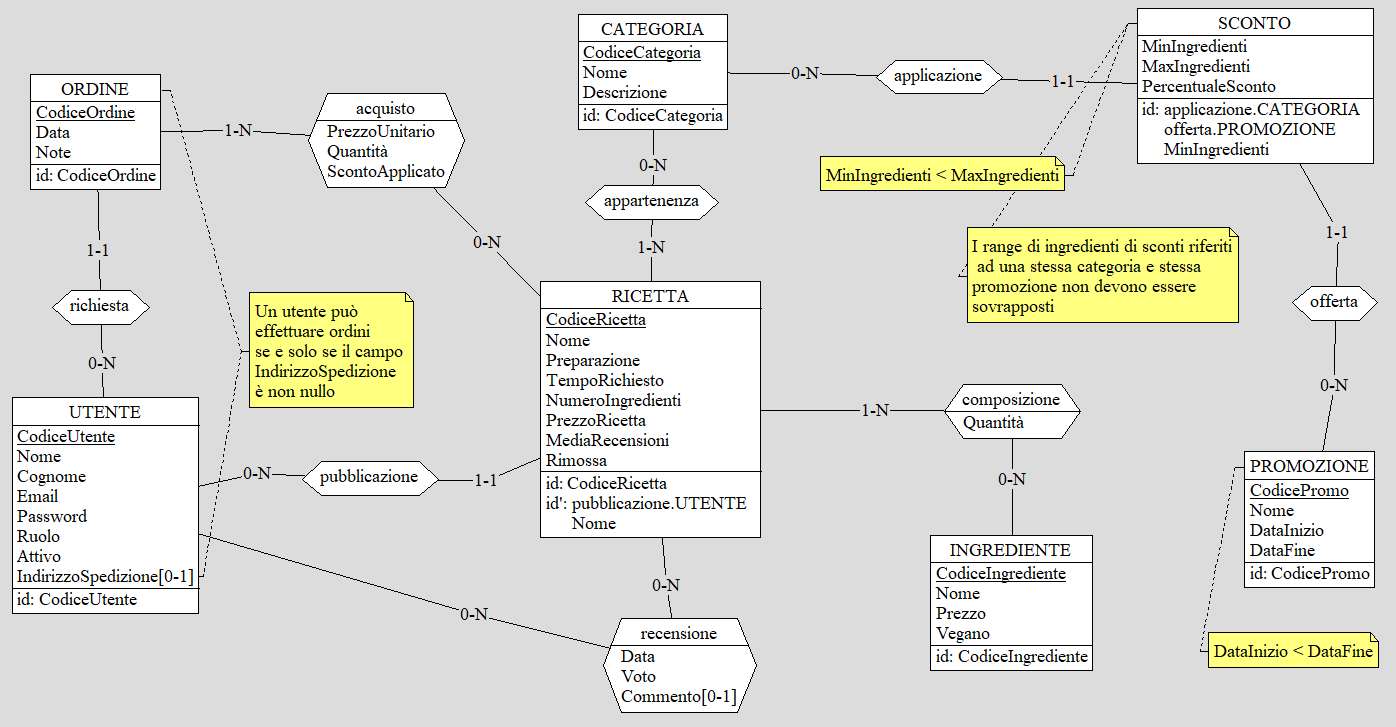
\includegraphics[width=1\textwidth]{images/conc_finale.png}
    \caption{Schema E/R completo.}
    \label{fig:conc_fin} % Etichetta per fare riferimento: vedi Figura \ref{fig:mia_immagine}
\end{figure}
\chapter{Progettazione logica}

\section{Stima del volume dei dati}

Si fornisce in questa fase una tabella contenente il numero medio di istanze di ogni entità e associazione dello schema concettuale finale.

\begin{table}[H]
\centering
\renewcommand{\arraystretch}{1.3} % Spaziatura comoda per le righe
\setlength{\tabcolsep}{10pt}     % Spaziatura orizzontale nelle celle

\begin{tabularx}{\textwidth}{|X|c|r|}
\hline
\textbf{Concetto} & \textbf{Tipo (E/R)} & \textbf{Volume} \\
\hline
UTENTE & E & 10.000 \\
\hline
pubblicazione & R & 150.000 \\
\hline
RICETTA & E & 150.000 \\
\hline
composizione & R & 1.500.000 \\
\hline
INGREDIENTE & E & 1.000 \\
\hline
appartenenza & R & 450.000 \\
\hline
CATEGORIA & E & 30 \\
\hline
richiesta & R & 300.000 \\
\hline
ORDINE & E & 300.000 \\
\hline
acquisto & R & 600.000 \\
\hline
PROMOZIONE & E & 1.000 \\
\hline
offerta & R & 15.000 \\
\hline
SCONTO & E & 15.000 \\
\hline
applicazione & R & 15.000 \\
\hline
recensione & R & 3.000.000 \\
\hline
\end{tabularx}
\caption*{\textbf{Tabella 3.1.1} - \textit{Tavola dei volumi del modello E/R.}}
\end{table}


\section{Descrizione delle operazioni principali e stima della loro frequenza}

In questa fase si propone una tavola delle operazioni utilizzata per costituire una stima delle principali
operazioni richieste da utenti standard e amministratori.

\begin{table}[H]
\centering
\renewcommand{\arraystretch}{1.3}
\setlength{\tabcolsep}{5pt} % Riduce leggermente lo spazio tra le colonne per far stare tutto

\small % Riduce leggermente la dimensione del testo per un layout più pulito

% Usiamo due colonne 'X' per bilanciare lo spazio tra Nome Operazione e Frequenza
\begin{tabularx}{\textwidth}{|c|>{\raggedright\arraybackslash}X|>{\raggedright\arraybackslash}X|c|}
\hline
\textbf{Codice Op.} & \textbf{Nome operazione} & \textbf{Frequenza} & \textbf{Tipo} \\
\hline
U1 & REGISTRAZIONE UTENTE & 5 al giorno & I \\
\hline
U2 & VISUALIZZAZIONE RICETTE & 300 al giorno & I \\
\hline
U3 & VISUALIZZAZIONE RICETTE PER FILTRO & (1000 utenti attivi) $\times$ 1 = 1000 al giorno & I \\
\hline
U4 & VISUALIZZAZIONE INGREDIENTI & 300 al giorno & I \\
\hline
U5 & PUBBLICAZIONE RECENSIONE & (1000 utenti attivi) $\times$ 0.1 = 100 al giorno & I \\
\hline
U6 & PUBBLICAZIONE RICETTA & 50 al giorno & I \\
\hline
U7 & VISUALIZZAZIONE VANTAGGI & (1000 utenti attivi) $\times$ 0.5 = 500 al giorno & I \\
\hline
U8.1 & VISUALIZZAZIONE MIGLIORI RICETTE IN BASE ALLE RECENSIONI & (1000 utenti attivi) $\times$ 1.5 = 1500 al giorno & I \\
\hline
U8.2 & VISUALIZZAZIONE MIGLIORI UTENTI & 10 al giorno & I \\
\hline
U8.3 & VISUALIZZAZIONE RICETTE PIÙ ORDINATE & (1000 utenti attivi) $\times$ 0.1 = 100 al giorno & I \\
\hline
U8.4 & VISUALIZZAZIONE CATEGORIE DI RICETTA PIÙ ORDINATE & (1000 utenti attivi) $\times$ 0.1 = 100 al giorno & I \\
\hline
U9 & EFFETTUAZIONE ORDINE & 100 al giorno & I \\
\hline
U10 & VISUALIZZAZIONE STORICO ORDINI & 50 al giorno & I \\
\hline
U11 & VISUALIZZAZIONE SPECIFICA RICETTA & (1000 utenti attivi) $\times$ 1.5 = 1500 al giorno & I \\
\hline
A1 & INSERIMENTO INGREDIENTE & 1 al mese & I \\
\hline
A2 & AGGIORNAMENTO INGREDIENTE & 5 a settimana & I \\
\hline
A3 & INSERIMENTO CATEGORIA & 1 all’anno & I \\
\hline
A4 & LANCIO PROMOZIONE & 5 all’anno & I \\
\hline
A5 & PUBBLICAZIONE SCONTO & 75 all’anno & I \\
\hline
A6 & RIMOZIONE UTENTI & 1 al mese & B \\
\hline
\end{tabularx}
\caption*{\textbf{Tabella 3.2.1} - \textit{Tavola delle operazioni del sistema.}}
\end{table}

\textbf{Nota}: la frequenza indicata nell’operazione U3 indica la frequenza totale di tutte le operazioni di ricerca per filtro (U3.1 - U3.6), le cui singole frequenze sono approssimativamente in ugual parti.
%\input{4_CommentiFinali}

%\appendix
%\titleformat{\chapter}[display]
%    {\normalfont\huge\bfseries}
%    {\appendixname~\thechapter}
%    {20pt}
%    {\Huge}
%\input{5_GuidaUtente}
%\input{6_EsercitazioniDiLaboratorio}

\end{document}